\section{Features}
Features bilden die Eingabe für einen Entscheidungsbaum. Gute Features sind integral, damit der Entscheidungsbaum gut generalisiert. Wenn die Featuremenge keine eindeutige Trennung der Klassen in der
Trainingsmenge zulässt, so ist auch keine gute Generalisierung zu erwarten.
\newline
\newline
In dieser Arbeit muss die Richtung der Handgeste klassifiziert werden. Die Handgeste kann mit verschiedenen Geschwindigkeiten und unterschiedlichen Distanzen zur Kamera durchgeführt werden. Mit
zunehmender Entfernung nimmt der Kontrast ab, da Streulicht einen größeren Einfluss hat. Für eine gute Generalisierung, sollten die Features Invarianzen zur Geschwindigkeit und den
Lichtverhältnissen haben. Erschwerend ist, dass die Handgeste nie exakt gleich ausgeführt wird. Sie kann eine leichte Kreisbewegungen aufweisen oder schräg durchgeführt werden, sodass einige
Fotowiderstände nicht verdeckt werden.
\subsection{Feature Verbesserungen}
Einige Anforderungen, können durch spezielle Änderungen an einem Feature ergänzt werden. Dazu gehören relative Helligkeitsunterschiede, Positionsinformationen und Entwicklung über die Zeit.
\newline
\newline
Relative Helligkeitsunterschiede können durch Normalisierung über die lokale Gesamthelligkeit eliminiert werden. Dadurch ändert sich aber die Art der Aussage über die absolute Helligkeit
zu einer Aussage über die relative Helligkeit. Das heißt, jeder Pixel in einem Bild wird durch die Summe der Pixel im Bild geteilt. Dies erzeugt eine Invarianz gegenüber der skalierten Helligkeiten,
jedoch nicht gegenüber Helligkeiten auf denen ein Offset addiert wurde.
\newline
\newline
Informationen über die Position können einerseits aus dem Argument des Features und andererseits durch partielle Anwendung inferiert werden. Beim Argument eines Features wird das Argument als Feature
bereitgestellt, indem das Feature bestimmte Bedingungen erfüllt. Bei $\arg(\max X)$ zum Beispiel, wird der Index bereitgestellt, an dem die Menge $X$ maximal ist. Bei der partiellen Anwendung wird das Feature auf
Teilmengen der Definitionsmenge angewendet und damit mehrfach zur Feature-Menge hinzugefügt, z. B. bei der Fotowiderstandmatrix könnten Zeilen und Spalten Teilmengen sein.
\newline
\newline
Die Entwicklung über Zeit kann ebenfalls über die Duplizierung des Features dargestellt werden. Anstatt einen einzelnen Bild zu unterteilen, wird die Handgeste in Zeitfenster aufgeteilt. Jedes Zeitfenster
fasst die einzelnen Bilder zu einem Bild zusammen. Für jedes Zeitfenster wird das Feature berechnet.
\subsection{Featureauswahl}
Insgesamt wurden 28 Varianten von Feature untersucht und davon 3 Feature verstärkt aus denen 20 Varianten entstanden sind. Die Features, die von Song et al. genutzt wurden
(siehe Tabelle \ref{tab:songFeatures}) eignen sich ohne Änderungen nicht, da sie mindestens eine Anforderung nicht erfüllen.
\newline
\newline
Mit dem \textit{Mean absolute value} ermöglicht es die einzelnen Handgesten zu unterscheiden, wenn das Feature in verschiedene Zeitfenster aufgeteil wird. Zusätzlich kann die Helligkeit normalisiert werden.
Um die Featuremenge zu verringern, können Spalten und Zeilen zusammengefasst werden. Allerdings generalisierte der Ansatz nicht gut, da die Varianz sehr groß ist durch die fehlende Invarianz zur Geschwindigkeit.
\newline
\newline
\textit{Average amplitude change} eignet sich gut um horizontale und vertikale Bewegungen zu unterscheiden. Allerdings ist es nicht möglich symethrische Bewegungen zu unterscheiden. Nicht untersucht wurden
Änderungen, die beim \textit{Mean absolute value} durchgeführt wurden.
\newline
\newline
Feature 2, 5, 7 bis 9 wurden nicht weiter untersucht weil sie zu komplexe Berechnungen bedürfen für das Arduino Board.

\subsubsection{Motion History}
Die Motion History zeigt eine Bewegunghistorie, indem kürzlich stattgefundene Bewegung heller ist als länger zurückliegende. Es ist invariant gegenüber Lichtverhältnisse, hat jedoch 2 große Schwachpunkte.
Einerseits kann es überlappende Bewegungen nicht richtig anzeigen, da eine kürzlich detektierte Bewegungung den Wert auf den Maximalwert $\tau$ setzt. Dies stellt in diesem Anwendungsfall kein
Problem dar, da die definierten Handgesten keine Überlappung erzeugen.
\newline
\newline
Andereseits ist das Feature bei konstantem $\tau$ und $\delta$ nicht Invariant gegenüber Geschwindigkeit. Als Lösung wurde $\delta$ abhängig von der Gestenlänge gemacht,
d. h. $\delta = \frac{\tau}{\#Bilder}$. Mit dieser Konfiguration ist die Bewegung nicht unvollständig, wenn sie langsam ausgeführt wird. Allerdings geht dieser Ansatz von einer konstanten
Ausführungsgeschwindigkeit der Handgeste aus.
\newline
\newline
Eine Bewegung in einem Pixel $q$ wird duch die Funktion \ref{formular:motion_history_phi} signalisiert, d. h. die Bewegung in $q$ findet statt, wenn eine Veränderung oberhalb des Durchschnitts detektiert wird.
\begin{align}
    \phi(q,t) = \begin{cases}
                    1 & if \Delta_{q,t} \geq \frac{1}{N} \sum_{n=1}^N \Delta_{q,n} \\
                    0 & otherwise
    \end{cases}
    \hspace{0.5cm}where\ \Delta_{q,t} = |q_t - q_{t-1}|
    \label{formular:motion_history_phi}
\end{align}

\subsubsection{Helligkeitsverteilung}
Ein Pixel $q$ ist am hellsten unter allen Pixeln in einem Bild $Q$, wenn $q$ den höchsten Wert hat. Analog ist der dunkelste Pixel, der mit dem geringsten Wert. Folglich kann der hellste Pixel als
$q' = \arg(\max Q)$, bzw. der dunkelste Pixel als $q' = \arg(\min Q)$ definiert werden.
\newline
\newline
Weiterhin wird die Bildsequenz in eine bestimmte Anzahl von gleich großen Zeitfenstern aufgeteilt. In jedem Zeitfenster wird der hellste bzw. dunkelste Pixel ermittelt. Aus der daraus resultierenden
Featuremenge kann jede definierte Handgeste inferiert werden. Sie ist invariant zu Lichtverhältnissen und Geschwindigkeiten. Per Definition gibt sie Auskunft über die Entwicklung über Zeit und die Position.
\newline
\newline
Es gibt mehrere Möglichkeiten die einzelnen Pixel in einem Zeitfenster zusammenzufassen.
\begin{itemize}
    \item Wähle das Minimum bzw. Maximum.
    \item Projeziere die Pixel auf ein kartesisches Koordinatensystem und fasse die Punkte über eine Abstandsmetrik zusammen, z. B. über den euklidischen Abstand.
    \item Unterteile die Pixel in Quadranten und wähle den Quadranten, der die meisten Einträge hat.
\end{itemize}
Außerdem können die Anzahl der Zeitfenster variiert werden und Pixel zu Gruppen zusammengefasst werden, d. h. Spalten und Zeilen.

\subsubsection{Schwerpunktverteilung}
\begin{figure}
    \centering
    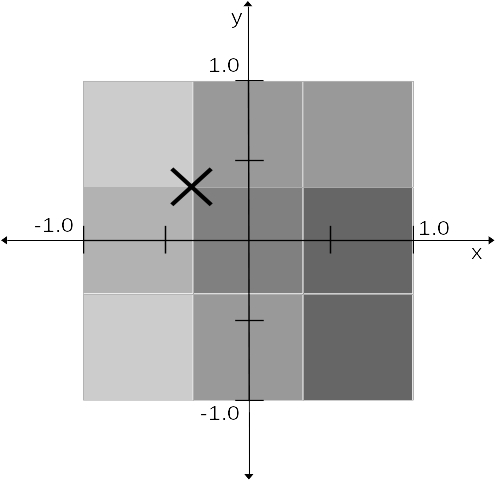
\includegraphics[width=0.5\linewidth]{images/schwerpunkt_ansatz.jpg}
    \caption{Illustration des Schwerpunktes im 3x3 Fotowiderstand-Array.}
    \label{fig:schwerpunkt}
\end{figure}
\begin{align}
    Q = \begin{pmatrix}
            q_{00} & q_{01} & q_{02} \\
            q_{10} & q_{11} & q_{12} \\
            q_{20} & q_{21} & q_{22}
    \end{pmatrix}
    \label{formular:pictureAsFormular}
\end{align}
Der Schwerpunkt $(X_Q, Y_Q)$ in einem Bild $Q$ (\ref{formular:pictureAsFormular}) ist über die Helligkeit in den einzelnen Pixel definiert. Der Pixel $q_{11}$ bildet den Nullpunkt des Koordinatensystems.
Dann ist relativ zur Gesamthelligkeit $P = \sum_{i,j} q_{i,j}$, $X_Q=\frac{\sum_{i=0}^{2} q_{i,2} - \sum_{i=0}^{2} q_{i,0}}{P}$ die horizontale Komponente
und $Y_Q = \frac{\sum_{i=0}^{2} q_{0,i} - \sum_{i=0}^{2} q_{2,i}}{P}$ die vertikale Komponente des Schwerpunktes \cite{schwerpunktAnsatz}.
\newline
\newline
Ähnlich zur Helligkeitsverteilung wird das Feature mit einer Zeithistorie erweitert durch die multiple Anwendung auf verschiedene Zeitfenster, wobei die Anzahl der Zeitfenster variiert werden kann. Die
einzelnen Schwerpunkte innerhalb eines Zeitfensters werden über den Durchschnitt zusammengefasst.
\newline
\newline
Sollte die Anzahl der Bilder einer Handgeste ein Vielfaches von der Anzahl der Zeitfenster sein, wird die gleiche Anzahl an Bilder auf jedes Zeitfenster verteilt. Ansonsten werden Überschüsse einem Muster
nach bestimmten Zeitfenstern zugeordnet. Bei 5 Zeitfenstern wird der erste Überschuss dem letzten Zeitfenster zugeordnet, der zweite dem ersten, der dritte dem dritten, der vierte dem zweiten.
\newline
\newline
Die Schwerpunktverteilung ist durch die Dividierung mit $P$ invariant gegenüber Skalierung der Helligkeit, jedoch nicht gegenüber einen Offset.
